\chapter{Implementazione}
\label{ch:implementazione} % This how you label a chapter and the key (e.g., ch:into) will be used to refer this chapter ``Introduction'' later in the report. 
% the key ``ch:into'' can be used with command \ref{ch:intor} to refere this Chapter.
parla di decomposizione delle funzionalità in microservizi
dipendenze minime tra i servizi
reattività agli eventi
\section{Tecnologie}
(-swagger, -postman, autogenerazione javadoc?, JWT per autenticazione utenti,
 docker, nodejs, typescript, mongodb, jest, angular, figma, ...)
\subsection{Swagger - OpenAPI}

Uno dei requisiti fondamentali di questo progetto è stata la documentazione delle API.
Per fare ciò è stato utilizzato Swagger, un framework open-source che permette di descrivere, produrre e consumare servizi web RESTful. 
Swagger permette di testare le API direttamente dalla documentazione, grazie a un'interfaccia grafica che consente di inviare richieste e visualizzare le risposte.

\vspace{1cm}

Per i servizi creati in Node.js è stata utilizzata una libreria ad hoc, in grado di generare la documentazione automaticamente tramite i corretti decoratori.
Al contrario, per i servizi in Java non esiste alcuna libreria in grado di generare automaticamente la documentazione API a partire dai metodi esposti, quindi è stata creata manualmente.
Grazie a un lavoro preliminare open-source svolto da \href{https://github.com/anupsaund}{\underline{Anup Saund}} sulla sua repository \href{https://github.com/anupsaund/vertx-auto-swagger}{\underline{Vertx auto swagger}}, è stato possibile creare automaticamente un file HTML contenente la documentazione delle API esposte dai servizi in Java. 
Purtroppo, questo file non era in grado di aggiornarsi automaticamente in caso di modifiche alle rotte, quindi è stato necessario adattarlo per renderlo più flessibile e adatto al nostro progetto.

\vspace{1cm}

Vertx è una libreria davvero completa e ben strutturata. È stato possibile creare un Router in grado di gestire tutte le rotte del progetto in Java utilizzando una semplice classe astratta che ha definito tutti i metodi utilizzati nel progetto, tramite la quale si è potuto razionalizzare il codice e creare dinamicamente la funzionalità richiesta.

\begin{lstlisting}[language=Java, caption={Semplice interfaccia per le rotte HTTP}, label=list:java_swagger_interface]
package httpRest;

import io.vertx.core.Handler;
import io.vertx.core.http.HttpMethod;
import io.vertx.ext.web.RoutingContext;

public interface IRouteResponse {
    HttpMethod getMethod();
    String getRoute();
    Handler<RoutingContext> getHandler();
}
\end{lstlisting}

La parte realmente complicata è stata fare in modo che le annotazioni presenti nel codice sorgente venissero lette e trasformate in un file JSON che rappresentasse correttamente la documentazione delle API. 
Dopo alcuni tentativi, è stato possibile automatizzare anche questa operazione.

\begin{lstlisting}[language=Java, caption={Aggiunta dei moduli delle classi contenenti rotte HTTP}, label=list:java_swagger_modules]
final ImmutableSet<ClassPath.ClassInfo> modelClasses = ImmutableSet.<ClassPath.ClassInfo>builder()
        .addAll(this.getClassesInPackage("game"))
        .addAll(this.getClassesInPackage("userModule"))
        .addAll(this.getClassesInPackage("BLManagement"))
        .addAll(this.getClassesInPackage("chatModule"))
        .build();
\end{lstlisting}

\vspace{1cm}

Java permette di creare oggetti molto complessi, diversi dai JSON / object solitamente utilizzati in JavaScript. Era fondamentale poter adoperare questi schemi per avere una documentazione ricca e per poter testare velocemente le API senza utilizzare necessariamente un client come Postman. 

Infine, per poter mostrare correttamente la documentazione, è stato necessario creare un file HTML che permettesse di visualizzare la documentazione in modo chiaro e ordinato. Questo file statico, presente nella repository del progetto, utilizza come fonte il file JSON di OpenAPI che viene rigenerato a ogni build del progetto, in modo da avere sempre la documentazione aggiornata.

\subsection{Postman}

Swagger ha semplificato lo sviluppo delle API e il loro funzionamento, ma non è sostenibile per testare chiamate API successive che seguono un certo ordine o che necessitano di payload specifici. Postman è stato fondamentale per risolvere questo problema.

È stata creata una raccolta di richieste, comodamente esportate da Swagger senza alcun bisogno di riscrittura. Queste possono contenere payload parametrizzati grazie alle variabili di ambiente settabili una volta per tutte, come ad esempio il GameID, che altrimenti, una volta creato, deve essere copiato e incollato in ogni richiesta successiva che lo richiede.

L'altro grande vantaggio di utilizzare Postman è stata la funzionalità Flows, che permette di creare un diagramma di flusso delle richieste e di salvare alcune risposte in variabili. Fino a quando non si è arrivati ad avere un frontend funzionante, questi Flows sono stati utili per trovare eventuali bug e avere ben chiaro il flusso di chiamate che sarebbero dovute essere implementate nel frontend, il che ha velocizzato lo sviluppo del frontend, seppur in minima parte.

E' stato realizzato un flow che simulasse la creazione di una partita, l'iscrizione di 4 giocatori, l'avvio della partita e la simulazione di un turno completo di gioco. Questo ha permesso di testare in modo spedito molte delle funzionalità del sistema, e di trovare eventuali bug in modo altrettanto rapido.

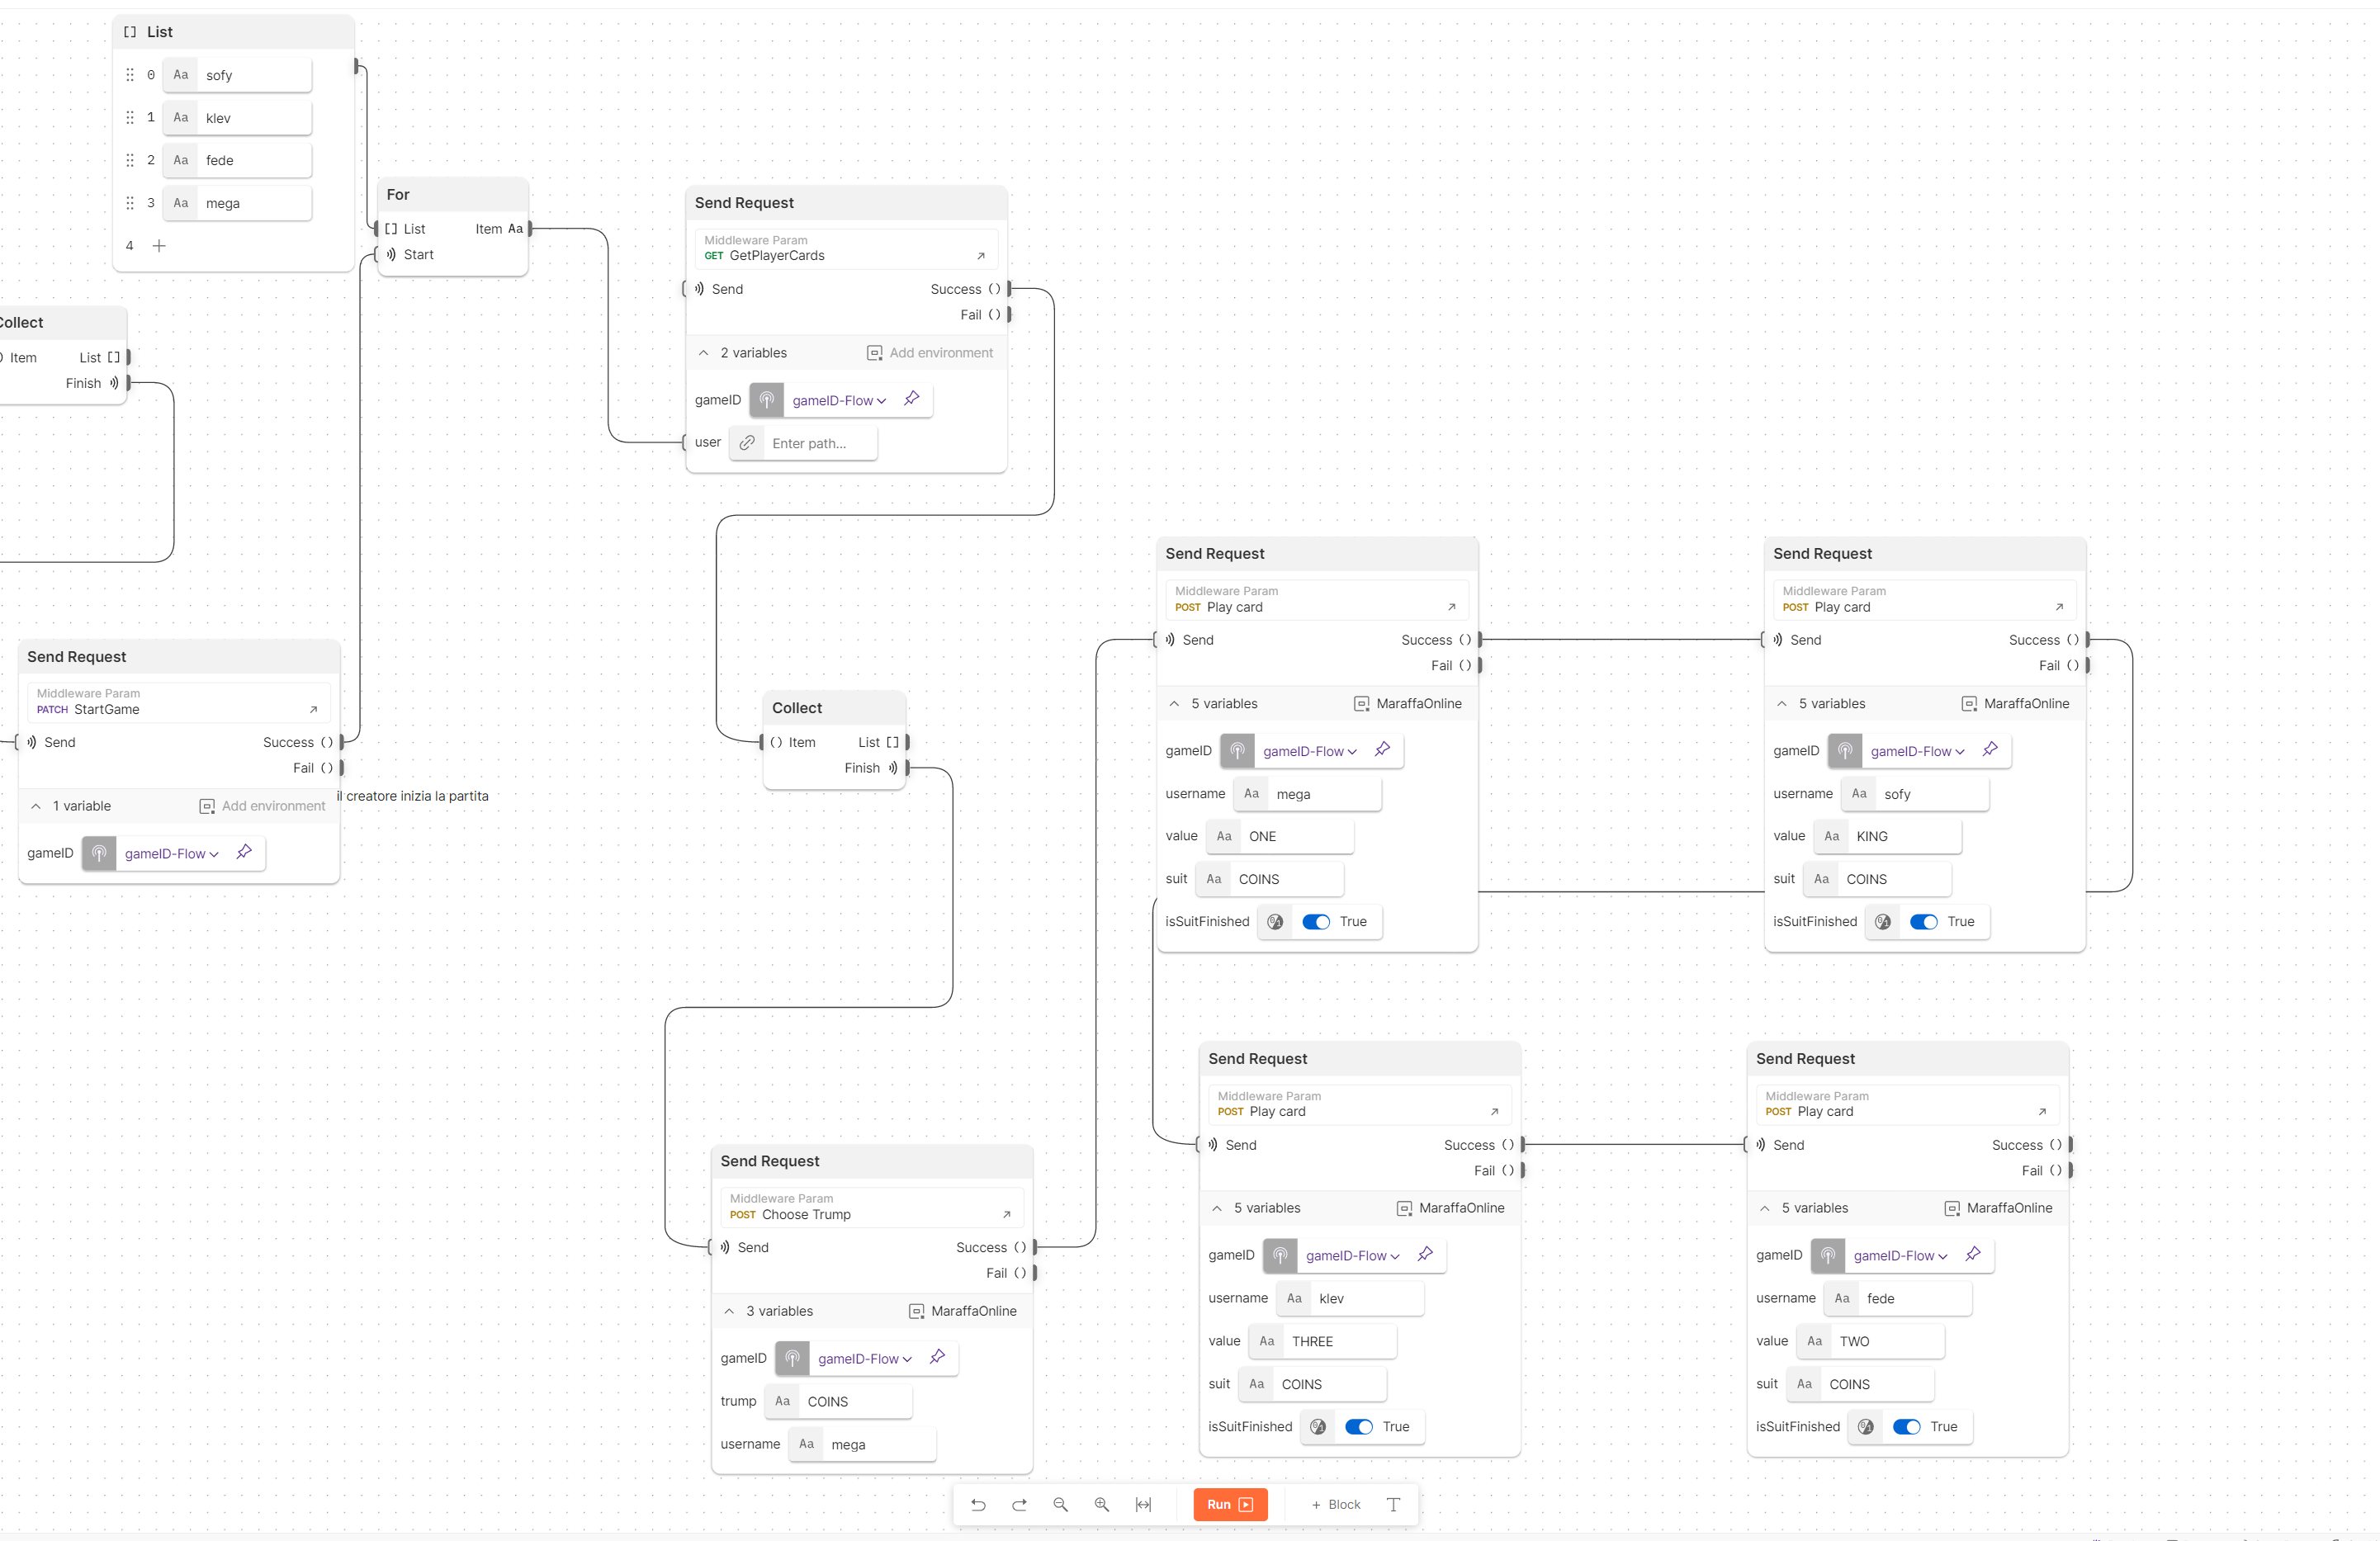
\includegraphics[width=18cm, height=10cm]{report/img/postManFlow.png}\\[15.5cm]


\subsection{Log automatici}

Il servizio core del sistema è il middleware e per poterlo monitorare è stato necessario implementare un sistema di log automatici. Tenere traccia di tutte le operazioni è un compito molto complesso e avrebbe reso difficile un eventuale debug su un software in produzione che in caso di errore potrebbe riavviarsi e perdere definitivamente quell'errore.
Grazie a Vertx, che offre "gratuitamente" un logger, e alla libreria \href{https://mvnrepository.com/artifact/ch.qos.logback/logback-classic}{\underline{LogBack}}, i log legati alle funzionalità più importanti sono trascritti su file .log in modo da poterli analizzare in caso di problemi.

Questo sistema poi si è evoluto grazie a una configurazione di LogBack in un file XML, tramite il quale è possibile personalizzare completamente il sistema di log, decidendo quali package loggare, in quali file trascriverli, scegliere il livello di log (info, debug, error, ecc.) e attuare un sistema di log rotate. Secondo questa configurazione, i log oltre una certa dimensione vengono compressi e rinominati per non occupare troppo spazio, e si può anche impostare il numero di questi file compressi da mantenere.

\begin{lstlisting}[language=Xml, caption={File configurazione Log automatici}, label=list:xml_logback]
    <appender name="DEBUG_LOG" class="ch.qos.logback.core.rolling.RollingFileAppender">
        <file>${DEBUG_FILE}</file>
        <rollingPolicy class="ch.qos.logback.core.rolling.SizeAndTimeBasedRollingPolicy">
            <fileNamePattern>${DEBUG_FILE}.%d{yyyy-MM-dd}.%i.gz</fileNamePattern>
            <maxFileSize>900MB</maxFileSize>
            <maxHistory>14</maxHistory>
            <totalSizeCap>2GB</totalSizeCap>
        </rollingPolicy>
        <encoder>
            <pattern>${LOG_PATTERN}</pattern>
        </encoder>
    </appender>


    <!-- Il package game usera la configurazione del log di debug -->
    <logger level="INFO" name="game" additivity="false">
        <appender-ref ref="DEBUG_LOG_ASYNC"/>
    </logger>

\end{lstlisting}

\vspace{1cm}

Questo sistema si adatta perfettamente a un software dockerizzabile che ha montato un volume relativo alla cartella /log, che può anche essere un volume remoto, da cui è possibile consultare velocemente i log in caso di problemi.

\begin{lstlisting}[language=Python, caption={Volume di log nel dockerfile l.13 da montare successivamente}, label=list:dockerfile_log]
FROM gradle:8.6.0-jdk17 AS build
COPY --chown=gradle:gradle . /home/gradle/src
WORKDIR /home/gradle/src
RUN gradle assemble
RUN gradle fatJar 

FROM openjdk:19

RUN mkdir /app
RUN mkdir /app/log

COPY --from=build /home/gradle/src/app/build/libs/ /app/
COPY --from=build /home/gradle/src/app/log /app/log

EXPOSE 3003
ENTRYPOINT ["java","-jar","/app/Middleware.jar"]
\end{lstlisting}

\section{Lettura varaibili d'ambiente TODO}
TODO
\section{Screen}
\section{Optional(Mockup)}
% %%%%%%%%%%%%%%%%%%%%%%%%%%%%%%%%%%%%%%%%%%%%%%%%%%%%%%%%%%%%%%%%%%%%%%%%%%%%%%%%%%%
% \section{Problem statement}
% \label{sec:intro_prob_art}
% This section describes the investigated problem in detail. You can also have a separate chapter on ``Problem articulation.''  For some projects, you may have a section like ``Research question(s)'' or ``Research Hypothesis'' instead of a section on ``Problem statement.'

% %%%%%%%%%%%%%%%%%%%%%%%%%%%%%%%%%%%%%%%%%%%%%%%%%%%%%%%%%%%%%%%%%%%%%%%%%%%%%%%%%%%
% \section{Aims and objectives}
% \label{sec:intro_aims_obj}
% Describe the ``aims and objectives'' of your project. 

% \textbf{Aims:} The aims tell a read what you want/hope to achieve at the end of the project. The  aims define your intent/purpose in general terms.  

% \textbf{Objectives:} The objectives are a set of tasks you would perform in order to achieve the defined aims. The objective statements have to be specific and measurable through the results and outcome of the project.


% %%%%%%%%%%%%%%%%%%%%%%%%%%%%%%%%%%%%%%%%%%%%%%%%%%%%%%%%%%%%%%%%%%%%%%%%%%%%%%%%%%%
% \section{Solution approach}
% \label{sec:intro_sol} % label of Org section
% Briefly describe the solution approach and the methodology applied in solving the set aims and objectives.

% Depending on the project, you may like to alter the ``heading'' of this section. Check with you supervisor. Also, check what subsection or any other section that can be added in or removed from this template.

% \subsection{A subsection 1}
% \label{sec:intro_some_sub1}
% You may or may not need subsections here. Depending on your project's needs, add two or more subsection(s). A section takes at least two subsections. 

% \subsection{A subsection 2}
% \label{sec:intro_some_sub2}
% Depending on your project's needs, add more section(s) and subsection(s).

% \subsubsection{A subsection 1 of a subsection}
% \label{sec:intro_some_subsub1}
% The command \textbackslash subsubsection\{\} creates a paragraph heading in \LaTeX.

% \subsubsection{A subsection 2 of a subsection}
% \label{sec:intro_some_subsub2}
% Write your text here...

% %%%%%%%%%%%%%%%%%%%%%%%%%%%%%%%%%%%%%%%%%%%%%%%%%%%%%%%%%%%%%%%%%%%%%%%%%%%%%%%%%%%
% \section{Summary of contributions and achievements} %  use this section 
% \label{sec:intro_sum_results} % label of summary of results
% Describe clearly what you have done/created/achieved and what the major results and their implications are. 


% %%%%%%%%%%%%%%%%%%%%%%%%%%%%%%%%%%%%%%%%%%%%%%%%%%%%%%%%%%%%%%%%%%%%%%%%%%%%%%%%%%%
% \section{Organization of the report} %  use this section
% \label{sec:intro_org} % label of Org section
% Describe the outline of the rest of the report here. Let the reader know what to expect ahead in the report. Describe how you have organized your report. 

% \textbf{Example: how to refer a chapter, section, subsection}. This report is organised into seven chapters. Chapter~\ref{ch:lit_rev} details the literature review of this project. In Section~\ref{ch:method}...  % and so on.

% \textbf{Note:}  Take care of the word like ``Chapter,'' ``Section,'' ``Figure'' etc. before the \LaTeX command \textbackslash ref\{\}. Otherwise, a  sentence will be confusing. For example, In \ref{ch:lit_rev} literature review is described. In this sentence, the word ``Chapter'' is missing. Therefore, a reader would not know whether 2 is for a Chapter or a Section or a Figure.
